\section{Introduction}
Le but de ce laboratoire est de réaliser un dépôt de Nickel électrolytique sur une pièce en laiton. Puis de mesurer l'épaisseur et la masse de la couche électrolytique à l'aide de trois méthodes différentes :

\begin{itemize}
    \item Par différence de masse
    \item Par mesure directe de l'épaisseur
    \item Par mesure de courant (loi de Faraday)
\end{itemize}

\section{Rappel théorique}
\subsection{le nickelage}

Le nickelage est un procédé de revêtement utilisé pour appliquer une couche de nickel sur une surface 
d'un autre matériau. Ce traitement est couramment utilisé pour améliorer l'apparence, la résistance
 à la corrosion, la dureté superficielle et la résistance à l'usure des pièces métalliques.\\
 Il existe trois méthodes pour réaliser le nickelage : méthode électrochimique (utilisé dans ce labo), chimique et par bain de nickel.
\subsection{Loi de Faraday}
La loi de Faraday pour l'électrolyse est donnée par l'équation suivante :

\begin{equation}\label{Equ:LoiFaraday}
m = \frac{M \cdot I \cdot t}{n \cdot F}
\end{equation}


où :

\begin{itemize}
  \item $m$ : masse de substance déposée [g]
  \item $M$ : masse molaire du métal [g/mol]
  \item $I$ : courant [A]
  \item $t$ : temps [s]
  \item $n$ : état d'oxydation des ions métalliques de la solution
  \item $F$ : constante de Faraday [C/mol], environ $96485$ C/mol
\end{itemize}

\section{Calculs}

\subsection{Surface de Nickelage}
\label{sec:SurfNick}
Les dimensions de notre échantillon ont été mesuré au pied à coulisse.
\begin{itemize}
    \item $L$ : 9,94 $\pm$ 0,01 mm
    \item $\ell$ : 9,95 $\pm$ 0,01 mm
    \item $h$ : 55,34 $\pm$ 0,01 mm
  \end{itemize} 
La surface total de notre échantillon est de: 
\begin{equation}
    S = 2 \cdot (L \cdot \ell + L \cdot h + \ell \cdot h) = 23,99 \pm 0,02 \space cm^2
\end{equation}

\subsection{Courant dans la cellule}
Dans le protocole de laboratoire, il a été demandé d'effectuer le dépôt,
avec une densité de courant $J$ de 40 à 50 $[mA/cm^2]$ pendant 30 minutes.

\vspace{0.3cm}

Avec la surface calculée ci-haut (voir §\ref{sec:SurfNick}), on obtient:
\begin{equation}
    I_{min} = J_{min} \cdot S = 0,04 \cdot 23,99 = 0,959 \space A
\end{equation}
\begin{equation}
    I_{max} = J_{max} \cdot S = 0,05 \cdot 23,99 = 1,200 \space A
\end{equation}
Le courant dans la cellule sera fixé à 1 Ampère.

\subsection{Masse théorique déposée}
Grâce à la loi de Faraday (eq. \ref{Equ:LoiFaraday}) on peut calculer la masse théorique
de dépôt de nickel.
    \begin{equation}
        m_{Ni} = \frac{M_{Ni} \cdot I \cdot t}{n_{Ni} \cdot F} = 0,547 \pm 0.027 g
    \end{equation}
    \begin{itemize}
        \item $m$ = 45,07 $\pm$ 0.01 g
        \item $M$ = 58,69 g/mol
        \item $I$ = 1 $\pm$ 0.05 A 
        \item $t$ = 1800 $\pm$ 5 s
        \item $n$ = 2
        \item $F$ = $96485$ C/mol
    \end{itemize}
  \subsection{épaisseur théorique déposée}
  En connaissant la masse volumique du nickel $\rho_{Ni}=8,900 g/cm^3$ on obtient le volume déposé :
  \begin{equation}
    V_{NiTh}=\frac{m_{NiTh}}{\rho_{Ni}}=\frac{0,547}{8,9}=0.061 \pm 0,003 cm^3 
  \end{equation} 
  On peut ensuite, avec la surface calculée, calculer l'épaisseur déposée en faisant l'hypothèse quelle est homogène sur toute la pièce. 
  \begin{equation}
    h_{Th}=\frac{V_{NiTh}}{S}=\frac{0.061}{23.99}=25.62\pm 1.28 \mu m
  \end{equation} 






\section{Calculs}
Afin de réaliser le nickelage de l'éprouvette, on a réalisé une série de mesures et de calculs afin de pouvoir déterminer le courant et la tension à régler selon la densité de courant demandé pour le nickelage.

\begin{table}[H]
    \centering
    \begin{tabular}{|l|l|}
    \hline
    \rowcolor[HTML]{CBCEFB} 
    Propriété & Valeur \\ \hline
    H {[}$mm${]} & 55,34 \\ \hline
    L1 {[}$mm${]} & 9,95 \\ \hline
    L2 {[}$mm${]} & 9,94 \\ \hline
    Masse {[}$g${]} & 45,07 \\ \hline
    \end{tabular}
    \caption{Dimensions de l'éprouvette}
    \label{tab: dimeprouv}
\end{table}



\begin{table}[H]
    \centering
    \begin{tabular}{|l|l|l|r|}
    \hline
    \rowcolor[HTML]{CBCEFB} 
    \textbf{} & \textbf{min} & \textbf{max} & \multicolumn{1}{l|}{\cellcolor[HTML]{CBCEFB}\textbf{Valeurs effectives}} \\ \hline
    I/S {[}mA/cm\textasciicircum{}2{]} & 40 & 50 & \multicolumn{1}{l|}{} \\ \hline
    I {[}mA{]} & 959,69248 & 1199,6156 & \cellcolor[HTML]{FFFF00}1000 \\ \hline
    R {[}Ohm{]} & 15 & 15 & \cellcolor[HTML]{FFFFFF} \\ \hline
    U {[}V{]} & 14,3953872 & 17,994234 & \cellcolor[HTML]{FFFF00}16,2 \\ \hline
    \end{tabular}
    \caption{Calculs du courant et de la tension}
    \label{tab: calculcourant}
    \end{table}


\section{Matériel et méthodes}

Pour réaliser ce Nickelage ainsi que les mesures qui en découlent, on a utilisé le matériel suivant :

\begin{itemize}[label=\textbullet]
    \item 1 éprouvette de laiton (à revêtir : cathode)
    \item 1 balance de précision 0.00 - 200.00 g
    \item 1 plaque de nickel (anode)
    \item 1 bêcher de 600 ml
    \item 1 verre de montre
    \item 500 ml d'électrolyte NiSO4
    \item 1 réchaud avec agitateur magnétique et thermostat, réglé sur 50 °C
    \item 1 transformateur 220 V AC / 0-25 V AC
    \item 1 redresseur 0-25 V AC / 0-20 V DC
    \item 1 ampèremètre
    \item 1 résistance 15 $\Omega$
    \item Fils de jonction avec fiches
    \item Petit matériel : tiges filetées, pinces crocodiles, etc.   
\end{itemize}

Le protocole réalisé pour ce laboratoire est le suivant :
\vspace{0.3cm}

On a commencé par nettoyer la pièce avec du papier abrasif et rincé à l'alcool en utilisant des gants pour ne pas graisser la pièce. Ensuite on a mesuré la pièce au pied à coulisse et pesé les échantillons.

\begin{figure}[H]
    \centering
    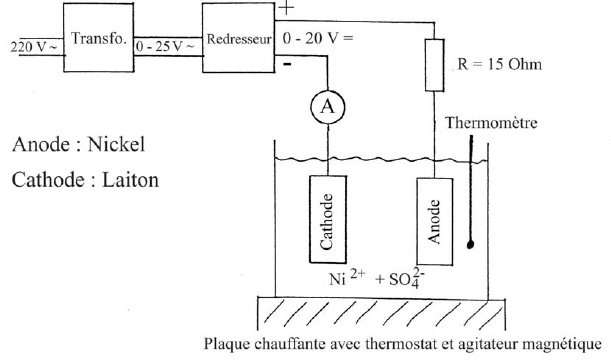
\includegraphics[width=12cm]{logos/schemamontage.png}
    \caption{Schéma de montage du bain de Nickelage électrochimique}
    \label{fig: montagesch}
\end{figure}

\vspace{0.3cm}
Après réalisation et contrôle du schéma de montage (Figure \ref{fig: montagesch}). On a réalisé le Nickelage avec un courant de 1A et 15 V (voir \ref{tab: calculcourant}), pendant 30 minutes.
Après réalisation et contrôle du schéma de montage (Figure \ref{fig: montagesch}). Nous avons réalisé le nickelage avec un courant de 1A et 15 V (voir \ref{tab: calculcourant}), pendant 30 minutes.

\vspace{0.3cm}
Après le nickelage, la pièce a été nettoyée à l'eau puis à l'alcool. Une nouvelle mesure de la masse de la pièce a ensuite été réalisée afin de déterminer l'épaisseur de la couche de nickel.

\vspace{0.3cm}
La préparation de l'échantillon s'est poursuivie avec une étape de tronçonnage, puis d'enrobage à chaud et finalement de polissage manuel selon le protocole de polissage manuel, voir annexe \ref{pdf: polissage}. Cela a permis par la suite d'observer l'épaisseur de la couche de nickelage au microscope optique.

\newpage
\section{Résultats}

\subsection{Par différence de masse}
\underline{Calcul de la section :}
\begin{equation}
    S = 2 \cdot (S_{section}+S_{hauteur1}+S_{hauteur2})
\end{equation}
\begin{center}
    $S = 2 \cdot (\text{L1} \cdot \text{L2} + \text{L1} \cdot \text{H} + \text{L2} \cdot \text{H}) $

    $S = 2 \cdot (9.95 \cdot 9.94 + 9.95 \cdot 55.34 + 9.94 \cdot 55.34) $
    
    \fbox{$S = 2399\ mm^2$}

\end{center}

\underline{Calcul de l'incertitude de la section :}

\begin{equation}\label{eq: incertitudeSection}
    \Delta S = 2 \cdot (\Delta S_{section} + \Delta S_{hauteur1} + \Delta S_{hauteur2})
\end{equation}

Or 

\begin{equation}
    \left(\frac{\Delta S_{surface}}{S_{surface}}\right)^2 = \left(\frac{\Delta X}{X}\right)^2 + \left(\frac{\Delta Y}{Y}\right)^2 
\end{equation}

\begin{equation}\label{eq: incertitudeSurface}
    \Delta S_{surface} = S_{surface} \cdot \sqrt{\left(\frac{\Delta X}{X}\right)^2 + \left(\frac{\Delta Y}{Y}\right)^2} 
\end{equation}


D'après l'équation \ref{eq: incertitudeSurface} on obtient :
\begin{itemize}
    \item $\Delta S_{section} = 9.95 \cdot 9.94\cdot \sqrt{\left(\frac{0.01}{9.95}\right)^2 + \left(\frac{0.01}{9.94}\right)^2}= 0.14 \text{ mm}^2$
    \item $\Delta S_{hauteur1} = 9.95 \cdot 55.34\cdot \sqrt{\left(\frac{0.01}{9.95}\right)^2 + \left(\frac{0.01}{55.34}\right)^2}= 0.56 \text{ mm}^2$
    \item $\Delta S_{hauteur2} = 9.94 \cdot 55.34\cdot \sqrt{\left(\frac{0.01}{9.94}\right)^2 + \left(\frac{0.01}{55.34}\right)^2}= 0.56 \text{ mm}^2$
\end{itemize}

\vspace{0.3cm}
D'après l'équation \ref{eq: incertitudeSection} on obtient :
\begin{equation}
    \Delta S = 2 \cdot (0.14 + 0.56 + 0.56) = 2.52 \text{ mm}^2 \text{ → } \text{\fbox{$3 \ mm^2$}}
\end{equation}

\underline{Données :}
\begin{itemize}
    \item Masse volumique du nickel : $\rho =$ 8900 $kg \cdot m^{-3}$ = 0.0089 $g \cdot mm^{-3}$
    \item Surface totale de l'échantillon : $S = 2399 \pm 3 \ mm ^2$
\end{itemize}


\begin{table}[H]
    \centering
    \begin{tabular}{|l|l|}
    \hline
    \rowcolor[HTML]{CBCEFB} 
    Propriété & Valeur [$g$]\\ \hline
    Masse avant nickelage & 45,07 \\ \hline
    Masse après nickelage  & 45,51 \\ \hline
    Masse de nickel déposée & 0,44 \\ \hline
    \end{tabular}
    \caption{Masse résultante du nickelage}
    \label{tab: masseNickel}
\end{table}

\underline{Calcul de l'incertitude sur la masse de nickel déposée :}
\begin{equation}
    \Delta m_{\text{depot}} = \Delta m_{\text{avant}} + \Delta m_{\text{après}} = 0.01 + 0.01 = 0.02 \text{ g}
\end{equation}

Ainsi \fbox{$m_{depot} =  0.44\ \pm$ 0.02 g}.

\vspace{0.6cm}
\underline{\normalfont{Calcul de l'épaisseur de la couche de nickel déposée :}}
\begin{equation}
    m_{depot} = h\cdot\rho\cdot S
\end{equation}
\begin{center}
    $h = \cfrac{m_{depot}}{\rho\cdot S} = \cfrac{0.44}{0.0089\cdot2399} = 0.0206 \ mm =$ \fbox{$20.6 \ \mu m$}
\end{center}




\underline{Calcul de l'incertitude sur l'épaisseur de la couche de nickel déposée :}
\begin{equation}
    \Delta h = h\cdot\sqrt{\left(\frac{\Delta m_{\text{depot}}}{m_{\text{depot}}}\right)^2 + \left(\frac{\Delta \rho}{\rho}\right)^2 + \left(\frac{\Delta S}{S}\right)^2}
\end{equation}

\begin{center}
    $\Delta h = h\cdot\sqrt{\left(\frac{0.02}{0.44}\right)^2 + \left(\frac{0}{0.0089}\right)^2 + \left(\frac{3}{2399}\right)^2}$
    \vspace{0.3cm}   

    $\Delta h = \num{0.9367e-3} \ mm = 0.937 \ \mu m $ \text{ → \fbox{$1\ \mu m$}}
\end{center}

Cette méthode nous donne une épaisseur de la couche de nickel déposée de 21 $\pm$ 1 $\mu m$. 

\subsection{Par mesure du courant}
\textcolor{red}{ajouter incertitude sur le temps et le courant}


En utilisant la formule \textcolor{red}{réf}, on obtient : 

\begin{equation}
    m_{nickel} = \frac{58,69 \cdot 1 \cdot 1800}{2 \cdot 96500} = 0.547 \text{ g}
\end{equation}

\subsection{Par mesure directe de l'épaisseur}
La mesure de l'épaisseur a été faite sur le microscope. Chaque 
photo a été prise au milieu d'un côté. On a fait une moyenne avec 
toutes les valeurs d'épaisseurs obtenues.  

\textcolor{red}{ajouter photos}

\textcolor{red}{ajouter tableau des valeurs}

\textcolor{red}{ajouter incertitude}



\section{Discussion des résultats}
Le dépot de nickel n'est pas uniforme d'une face à l'autre et cela est dû à la position de l'éprouvette dans le bain de nickelage. La face de l'éprouvette qui se trouve la plus proche de l'anode reçoit plus de nickel que l'autre face. En effet, la densité de courant est plus élevée à proximité de l'anode.



\subsection{Avantages et inconvénients des méthodes de mesure}
\subsubsection{Par différence de masse}
\textbf{Avantages méthode différence de masse :}
\begin{itemize}
    \item Facile à réaliser
    \item Mesure précise de la masse
    \item Pas besoin de matériel très spécifique
    \item Pas de risque de perte de matière
\end{itemize}

\textbf{Inconvénients méthode différence de masse :}
\begin{itemize}
    \item Estimation de l'épaisseur en passant par la masse volumique et la surface de l'échantillon
\end{itemize}

\subsubsection{Par mesure du courant}
\textbf{Avantages méthode mesure du courant :}
\begin{itemize}
    \item ?
\end{itemize}

\textbf{Inconvénients méthode mesure du courant :}
\begin{itemize}
    \item ?
\end{itemize}


\subsubsection{Par mesure directe de l'épaisseur}
\textbf{Avantages méthode mesure directe de l'épaisseur :}
\begin{itemize}
    \item Précis
\end{itemize}

\textbf{Inconvénients méthode mesure directe de l'épaisseur :}
\begin{itemize}
    \item Risque de perte de matière à la préparation
    \item Temps de préparation de l'échantillon
    \item Nécessite un microscope optique
\end{itemize}


\section{Conclusion}
